\section{Systembeskrivelse}
Til projektet er der anvendt det tildelte pan tilt system som har påmonteret de 2 hall sensorer samt h-broer som styrer motorerne som sidder på hhv pan og tilt.\\
Til at styre denne opsætning er der udleveret èt stk Field Programmable Gate Array (FPGA) og èn Microprocessor unit.
\\
På FPGA'en \cite{Nexys2Datasheet} er der 4 knapper, 8 switches, og 4 7-segment displays som bliver anvendt i projektet.

Det udleverede LaunchPad board fra Texas Instruments har påmonteret en TM4C123GH6PM Arm Cortex M4 Micro Processor Unit (MPU)\cite{TM4C123GH6PMDatasheet}.

\begin{figure}[!ht]
	\begin{center}
		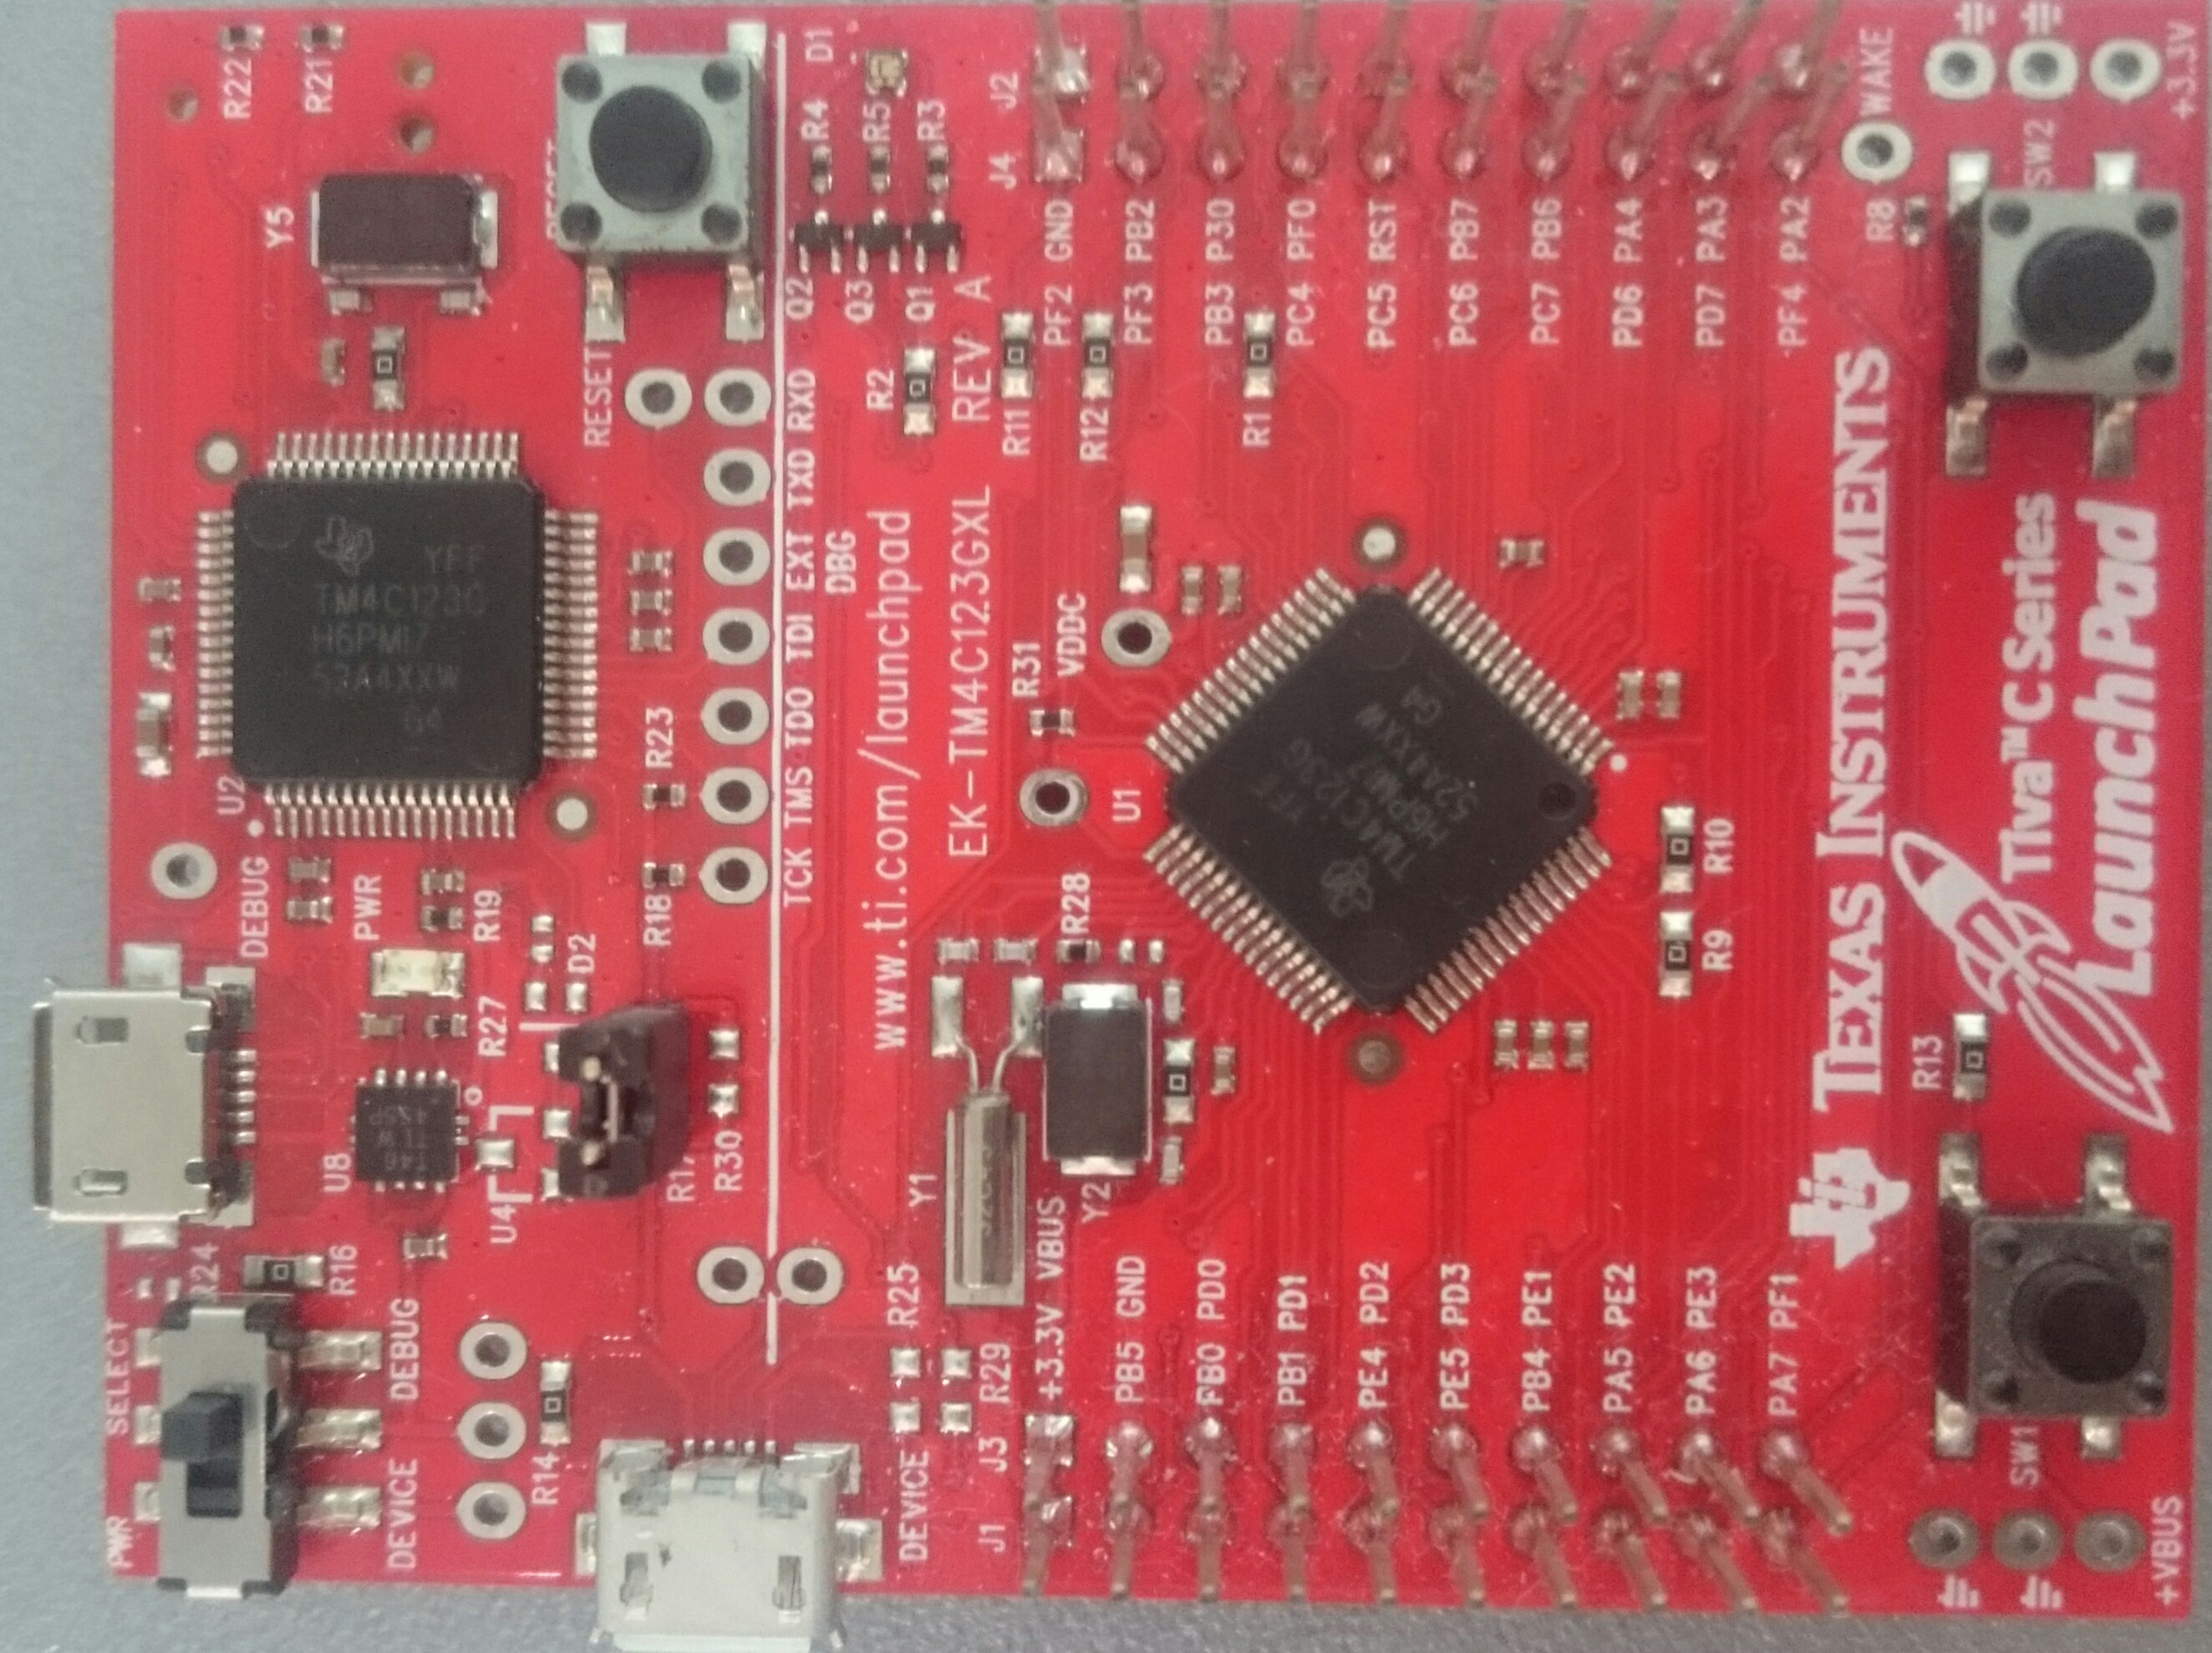
\includegraphics[scale=0.1, angle =270]{Billeder/TivaLaunchPad.JPG}
	\end{center}
\caption{Tiva Launch pad boardet med den tilføjede TM4C123GH6PM arm cortex M4 Micro Processor Unit}
\label{fig:TivaLaunchPad}
\end{figure}

Launch pad boarded kan tilføjes til et EMP board som blev udleveret i starten af semesteret som inkluderer et keypad, et lcd og en drehimpulsgeber, samt en SPI udgang som bliver anvendt, se figur XXXXX evt reference til datablad

\begin{figure}[!ht]
	\begin{center}
		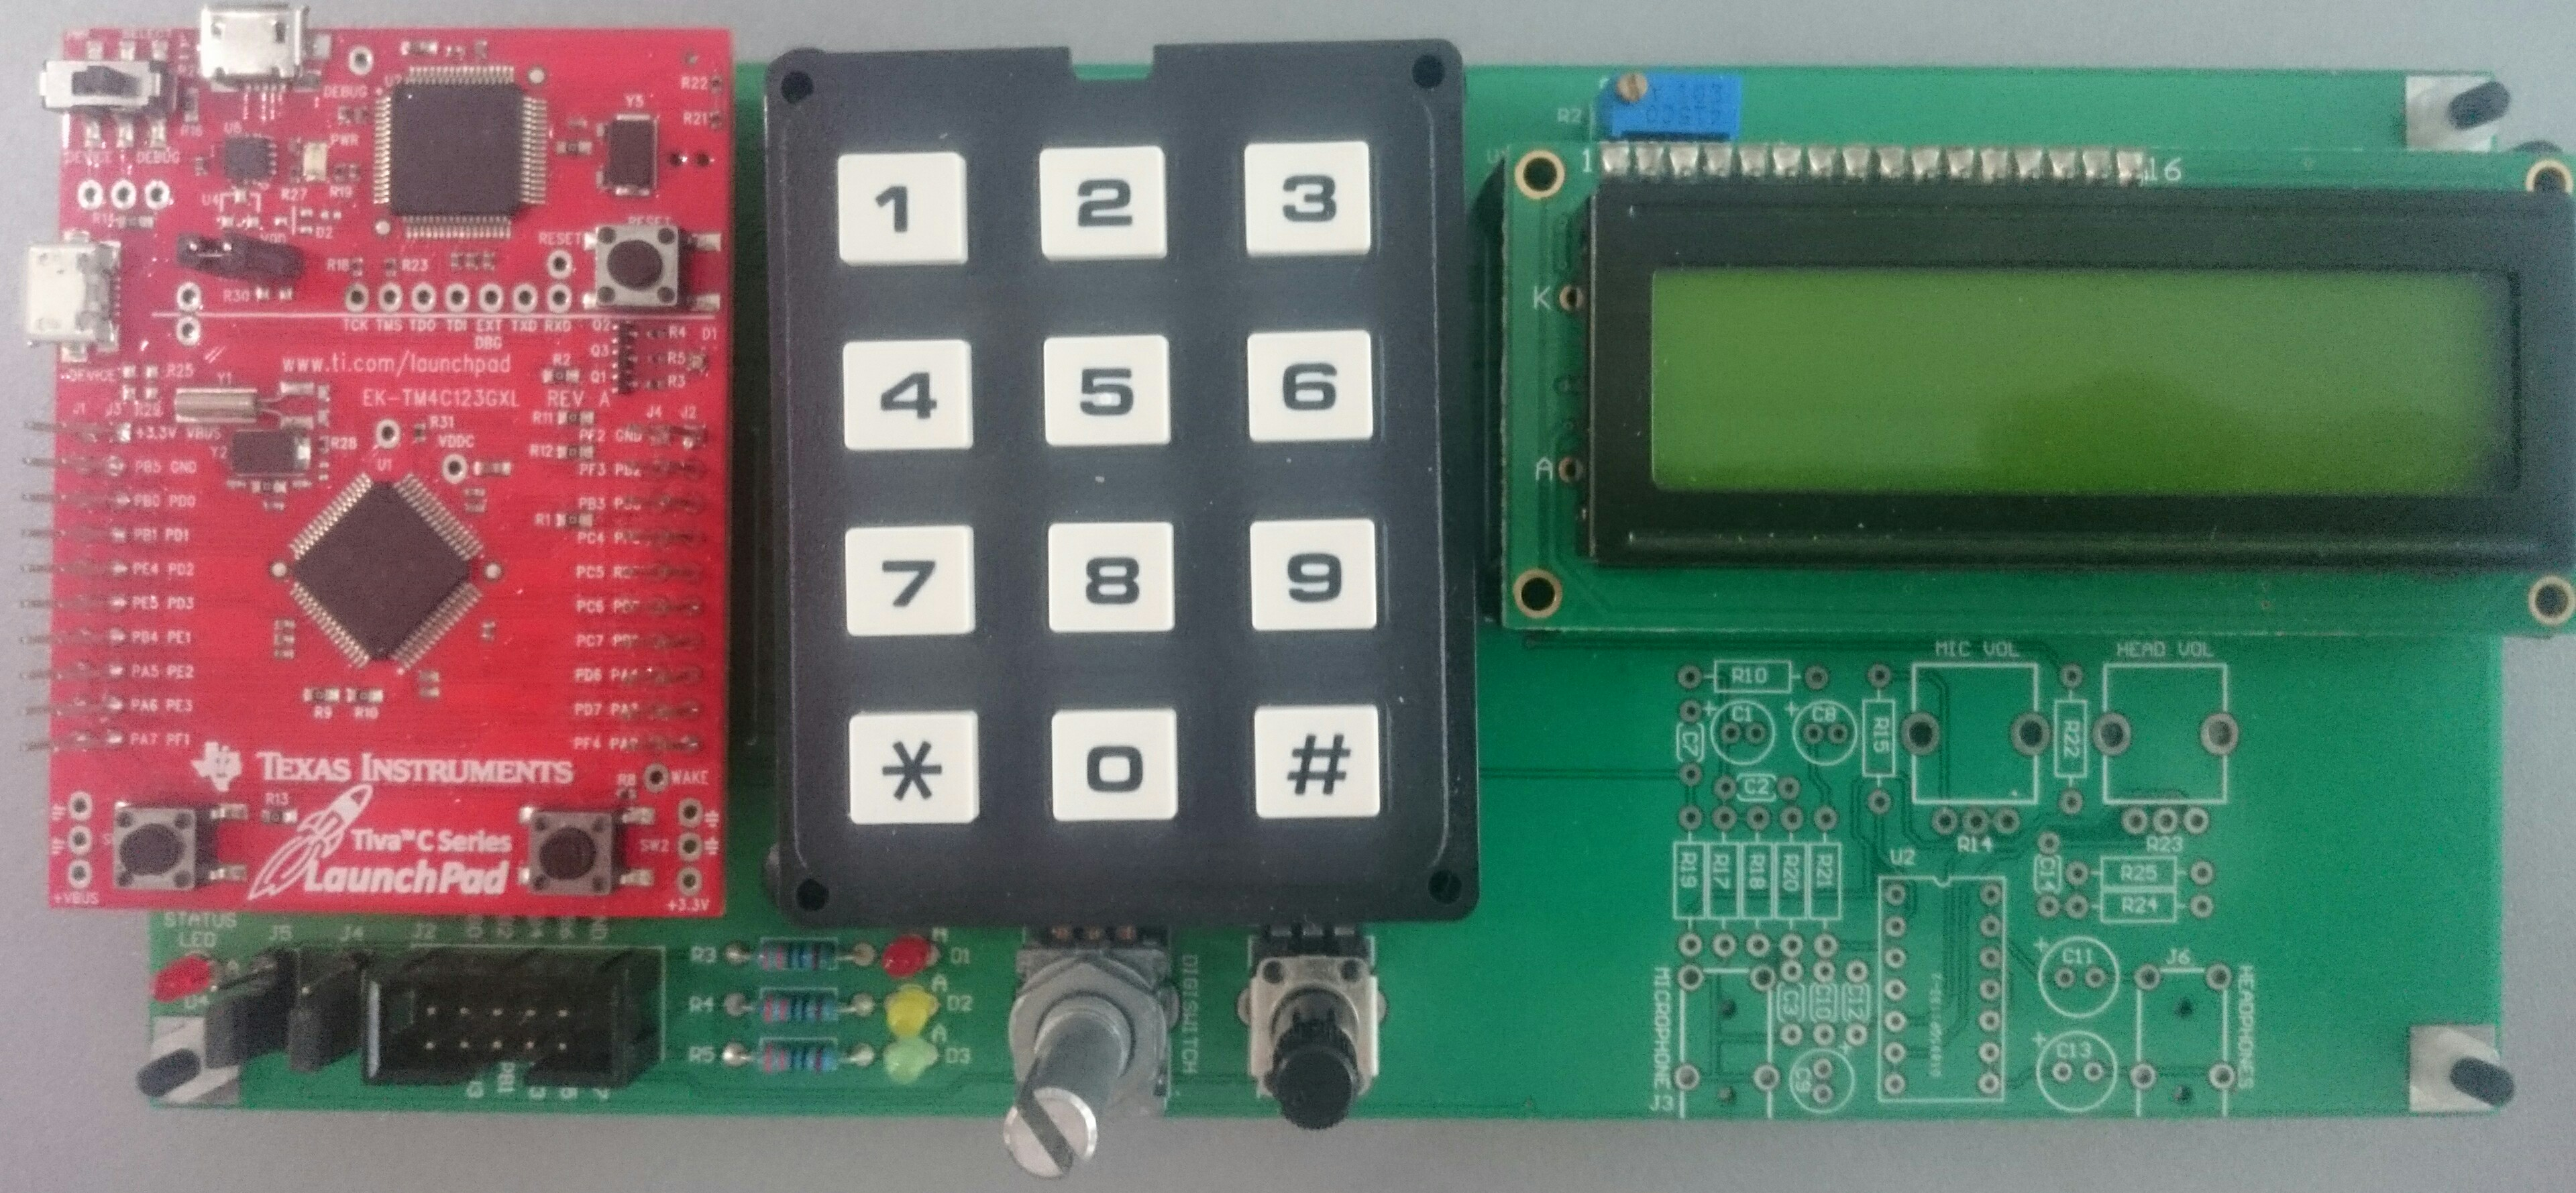
\includegraphics[scale=0.1, angle =0]{Billeder/EMP_BOARD.JPG}
	\end{center}
\caption{EMP Board med det tilføjede Launch pad board}
\label{fig:EMP_BOARD}
\end{figure}

FPGA'en vil styre motorerne med et Pulse-width modulation (PWM) signal som sendes til h-broerne som bestemmer hvilken retning strømmen skal sendes til motoren så de både kan køre med og mod uret.


%Besskrive hvorfra vi år koordinatsættet (hvor på nettet)